\begin{figure}[t]
\hspace{-3pt}
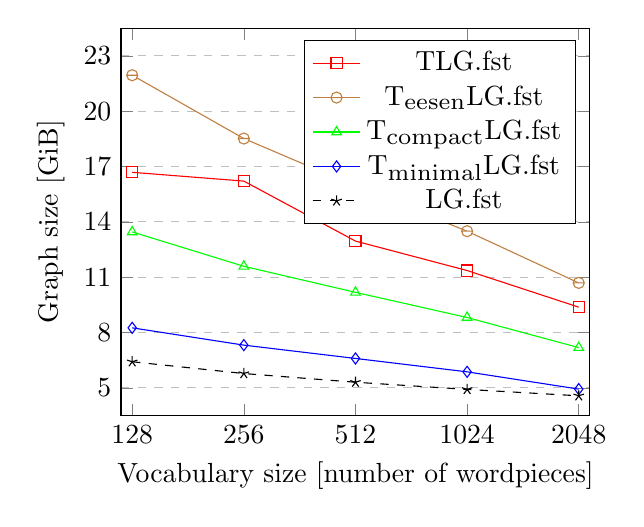
\begin{tikzpicture}
\pgfplotsset{%
    x tick label style={/pgf/number format/1000 sep=\,},
    log base 10 number format code/.code={%
        $\pgfmathparse{10^(#1)}\pgfmathprintnumber{\pgfmathresult}$%
    }%
}  
\begin{axis}[
    xmode=log,
    log ticks with fixed point,
    xlabel={Vocabulary size [number of wordpieces]},
    ylabel={Graph size [GiB]},
    height=6.5cm,
    xmin=128, xmax=2048,
    ymin=4, ymax=24,
    xtick={128,256,512,1024,2048},
    xticklabels={128,256,512,1024,2048}, % latex incorrectly displays logarithmic ticks
    ytick={5,8,11,14,17,20,23},
    legend pos=north east,
    ymajorgrids=true,
    grid style=dashed,
	enlargelimits=0.025,
]

\addplot[
    color=red,
    mark=square,
    ]
    coordinates {
    (128,16.686580021)(256,16.210114081)(512,12.958632869)(1024,11.360642777)(2048,9.374569253)};
    \addlegendentry{TLG.fst}

\addplot[
    color=brown,
    mark=halfcircle,
    ]
    coordinates {
    (128,21.951218701)(256,18.518031621)(512,15.936703145)(1024,13.494135421)(2048,10.690085437)};
    \addlegendentry{T\textsubscript{\scalebox{1.2}{eesen}}LG.fst}

\addplot[
    color=green,
    mark=triangle,
    ]
    coordinates {
    (128,13.454113621)(256,11.590339129)(512,10.177699053)(1024,8.813753657)(2048,7.180788233)};
    \addlegendentry{T\textsubscript{\scalebox{1.2}{compact}}LG.fst}

\addplot[
    color=blue,
    mark=diamond,
    ]
    coordinates {
    (128,8.253983465)(256,7.316065853)(512,6.594173965)(1024,5.867700781)(2048,4.931680801)};
    \addlegendentry{T\textsubscript{\scalebox{1.2}{minimal}}LG.fst}

\addplot[
    color=black,
    mark=star,
    dashed]
    coordinates {
    (128,6.414693433)(256,5.775879145)(512,5.303925905)(1024,4.915517181)(2048,4.568019881)};
    \addlegendentry{LG.fst}

\end{axis}
\end{tikzpicture}
%\vspace{-25pt} % adjust this
\vspace{-20pt} % adjust this
\caption{Decoding graph sizes with the considered topologies.}
\label{fig:graph-plot}
\vspace{-15pt} % adjust this
\end{figure}


% data
% correct: arcs[769667056,763880501,615276649,546992982,458390283] states[218595353,199401300,155710321,130437750,102016233] size[16686580021,16210114081,12958632869,11360642777,9374569253]
% eesen: arcs[850391361,725126731,630790485,540320351,433968267] states[417247843,345800193,292202766,242450487,187329655] size[21951218701,18518031621,15936703145,13494135421,10690085437]
% no selfloops: arcs[652025108,664179852,529217612,473743121,399820617] states[218595353,199401300,155710321,130437750,102016233] size[14804308853,14614903697,11581688277,10188645001,8437454597]
% compact: arcs[568826531,497023424,442389958,388478692,321522093] states[217644453,181898214,154972983,129904726,101821734] size[13454113621,11590339129,10177699053,8813753657,7180788233]
% minimal: arcs[368821525,332628298,304562070,275168966,235017961] states[117641950,99700651,86059039,73249863,58569668] size[8253983465,7316065853,6594173965,5867700781,4931680801]
% LG: arcs[252984303,235332235,222307595,211601871,202026046] states[118347226,100528166,87350216,76494359,66780154] size[6414693433,5775879145,5303925905,4915517181,4568019881]